\documentclass[border=12pt,crop=true]{standalone}
\usepackage{tikz}
\usetikzlibrary{positioning,arrows.meta}

\begin{document}
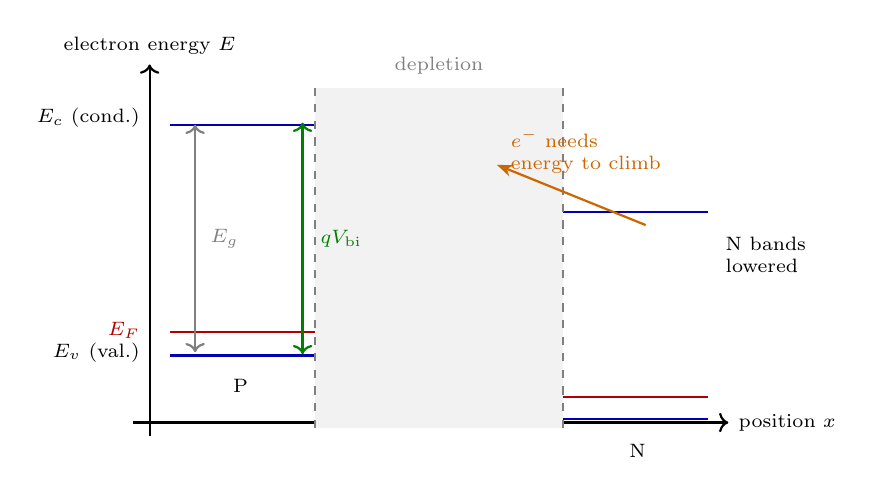
\begin{tikzpicture}[font=\small, x=1.05cm, y=0.85cm]

  \def\boxTop{5.0}
  \def\depL{2.0}
  \def\depR{5.0}

  % axes
  \draw[->, thick] (-0.2,0) -- (7.0,0) node[right, font=\scriptsize] {position $x$};
  \draw[->, thick] (0,-0.2) -- (0,\boxTop+0.35)
    node[above, font=\scriptsize] {electron energy $E$};

  \node[font=\scriptsize, anchor=east] at (0,4.55) {$E_c$ (cond.)};
  \node[font=\scriptsize, anchor=east] at (0,1.05) {$E_v$ (val.)};
  \node[font=\scriptsize, red!70!black, anchor=east] at (0,1.38) {$E_F$};

  % P flat bands
  \draw[thick, blue!70!black] (0.25,4.45) -- (\depL,4.45);
  \draw[thick, blue!70!black] (0.25,1.0) -- (\depL,1.0);
  \draw[red!70!black, thick] (0.25,1.35) -- (\depL,1.35);
  \node[font=\scriptsize] at (1.1,0.55) {P};

  % N flat bands (lowered)
  \draw[thick, blue!70!black] (\depR,3.15) -- (6.75,3.15);
  \draw[thick, blue!70!black] (\depR,0.05) -- (6.75,0.05);
  \draw[red!70!black, thick] (\depR,0.38) -- (6.75,0.38);
  \node[font=\scriptsize] at (5.9,-0.42) {N};

  % bending in depletion
  \draw[thick, blue!70!black] (\depL,4.45) .. controls (3.15,4.15) and (3.85,3.55) .. (\depR,3.15);
  \draw[thick, blue!70!black] (\depL,1.0) .. controls (3.15,0.96) and (3.85,0.62) .. (\depR,0.05);
  \draw[red!70!black, thick] (\depL,1.35) .. controls (3.15,1.31) and (3.85,0.68) .. (\depR,0.38);

  % depletion
  \fill[gray!10] (\depL,-0.08) rectangle (\depR,\boxTop);
  \draw[dashed, gray] (\depL,-0.08) -- (\depL,\boxTop);
  \draw[dashed, gray] (\depR,-0.08) -- (\depR,\boxTop);
  \node[font=\scriptsize, gray, anchor=south] at (3.5,\boxTop+0.05) {depletion};

  % band gap on P side
  \draw[<->, gray, thick] (0.55,1.05) -- (0.55,4.45);
  \node[font=\scriptsize, gray, anchor=west] at (0.62,2.75) {$E_g$};

  % barrier height
  \draw[<->, thick, green!50!black] (1.85,4.48) -- (1.85,1.02);
  \node[font=\scriptsize, green!50!black, anchor=west] at (1.95,2.75)
    {$qV_{\mathrm{bi}}$};

  % electron blocked (schematic)
  \draw[-{Stealth[length=2mm]}, thick, orange!80!black] (6.0,2.95)
    .. controls (5.2,3.35) .. (4.2,3.85);
  \node[font=\scriptsize, orange!80!black, align=left, anchor=west]
    at (4.25,4.05) {$e^-$ needs\\energy to climb};

  \node[font=\scriptsize, align=left, anchor=west] at (6.85,2.5)
    {N bands\\lowered};

\end{tikzpicture}
\end{document}
